\documentclass{article}
\usepackage{listings}
\usepackage{graphicx}

\title{Ejercicio 4: Salpicadero}
\begin{document}

\maketitle

\begin{figure}[h]
    \centering
    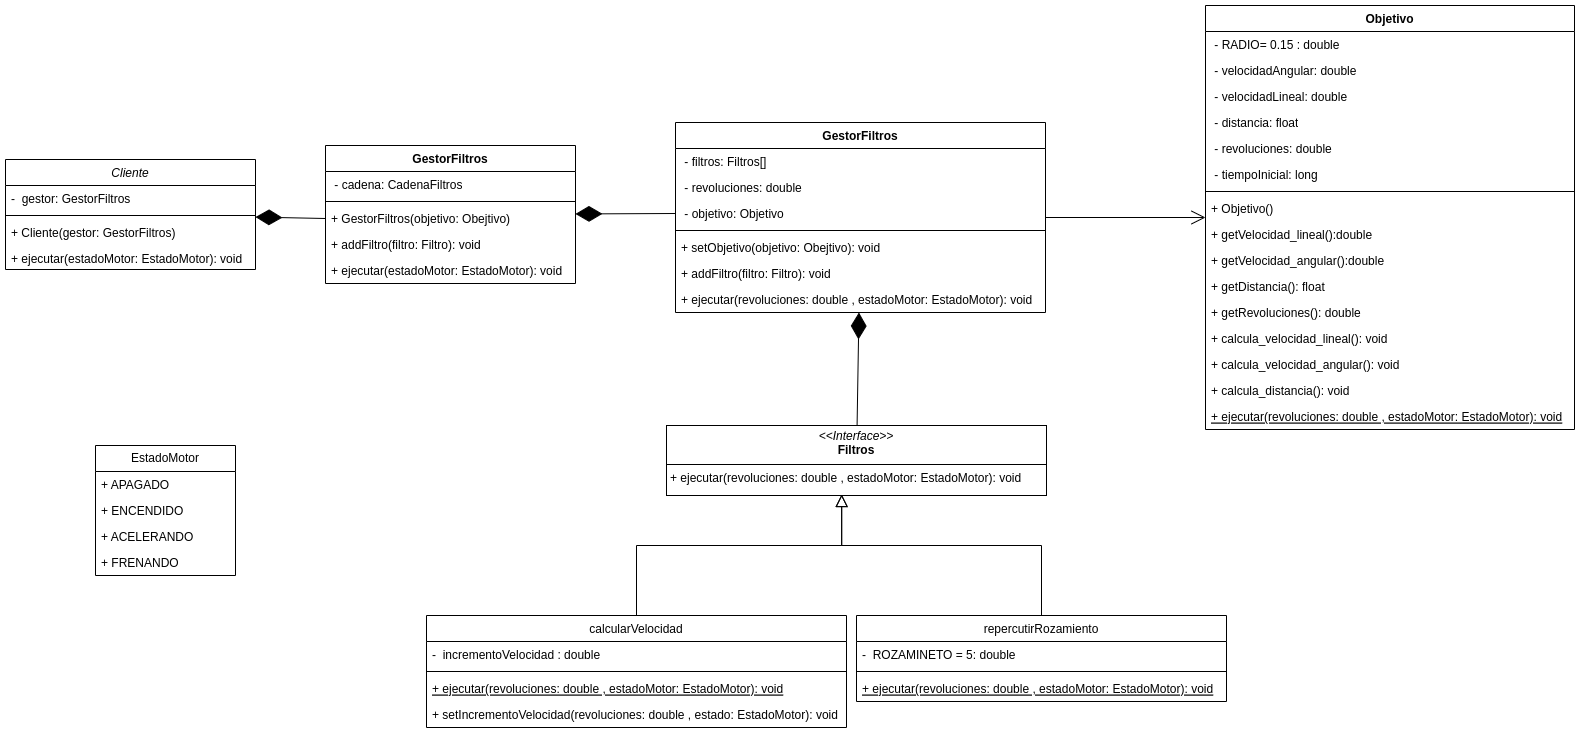
\includegraphics[width=1.2\textwidth]{Ej4_Practica1_DS.png}
    \caption{Diagrama de clase.}
    \label{fig:ejemplo}
\end{figure}

\section{Clase Cliente}

La clase \texttt{Cliente} representa un cliente que utiliza un \texttt{GestorFiltros} para establecer las revoluciones del motor apartir de un estado que se le pase.

\begin{lstlisting}

\noindent Los atributos de la clase incluyen:

\begin{itemize}
    \item \texttt{gestor:} el gestor de filtros utilizado por el cliente.
\end{itemize}

\noindent\textbf{public Cliente(GestorFiltros g)}

Constructor de la clase \texttt{Cliente} que recibe un \texttt{GestorFiltros} como parámetro y lo asigna al atributo \texttt{gestor}.

\begin{itemize}
    \item \textbf{g:} el gestor de filtros a asignar.
\end{itemize}

\noindent\textbf{public void ejecutar(EstadoMotor estadoMotor)}

Método que ejecuta los filtros en el motor utilizando el gestor de filtros asignado.

\begin{itemize}
    \item \textbf{estadoMotor:} el estado actual del motor.
\end{itemize}

\end{lstlisting}
%#############################################################################################################################################

\section{Clase GestorFiltros}

La clase \texttt{GestorFiltros} gestiona una cadena de filtros y proporciona métodos para agregar filtros y ejecutarlos en un motor.

\begin{lstlisting}

\noindent Los atributos de la clase incluyen:

\begin{itemize}
    \item \texttt{cadena:} la cadena de filtros administrada por el gestor.
\end{itemize}

\noindent\textbf{public GestorFiltros(Objetivo o)}

Constructor de la clase \texttt{GestorFiltros} que recibe un \texttt{Objetivo} como parámetro y que se lo pasa a \texttt{CadenaFiltros} 

\begin{itemize}
    \item \textbf{o:} el objetivo al que se aplicarán los filtros.
\end{itemize}

\noindent\textbf{public void addFiltro(Filtro f)}

Agrega un filtro a la cadena de filtros administrada por el gestor.

\begin{itemize}
    \item \textbf{f:} el filtro que se añade a la cadena.
\end{itemize}

\noindent\textbf{public void ejecutar(EstadoMotor estadoMotor)}

Ejecuta la cadena de filtros en el motor.

\begin{itemize}
    \item \textbf{estadoMotor:} el estado actual del motor.
\end{itemize}

\end{lstlisting}

%#######################################################################################################################################

\section{Clase CadenaFiltros}

La clase \texttt{CadenaFiltros} gestiona una lista de filtros y proporciona métodos para agregar filtros, establecer un objetivo y ejecutar los filtros en un motor.

\begin{lstlisting}

\noindent Los atributos de la clase incluyen:

\begin{itemize}
    \item \texttt{filtros:} una lista de filtros.
    \item \texttt{objetivo:} el objetivo al que se aplicarán los filtros.
    \item \texttt{revoluciones:} las revoluciones actuales del motor.
\end{itemize}

\noindent\textbf{public void addFiltro(Filtro f)}

Agrega un filtro a la lista de filtros.

\begin{itemize}
    \item \textbf{f:} el filtro a agregar.
\end{itemize}

\noindent\textbf{public void setObjetivo(Objetivo o)}

Establece el objetivo al que se aplicarán los filtros.

\begin{itemize}
    \item \textbf{o:} el objetivo a establecer.
\end{itemize}

\noindent\textbf{public void ejecutar(EstadoMotor estadoMotor)}

Ejecuta la lista de filtros en el motor y, opcionalmente, ejecuta el objetivo.

\begin{itemize}
    \item \textbf{estadoMotor:} el estado actual del motor.
\end{itemize}

\end{lstlisting}

%##########################################################################################################################################

\section{Interfaz Filtro}

La interfaz \texttt{Filtro} define un método para ejecutar filtros en un motor.

\begin{lstlisting}

\noindent\textbf{public double ejecutar(double revoluciones, EstadoMotor estadoMotor)}

Método que ejecuta un filtro en el motor.

\begin{itemize}
    \item \textbf{revoluciones:} las revoluciones actuales del motor.
    \item \textbf{estadoMotor:} el estado actual del motor.
    \item \textbf{Return:} el resultado de aplicar el filtro.
\end{itemize}

\end{lstlisting}


%#############################################################################################################################################

\section{Clase FiltroCalcularVelocidad}

La clase \texttt{FiltroCalcularVelocidad} implementa la interfaz \texttt{Filtro} y proporciona métodos para calcular la velocidad de un motor.

\begin{lstlisting}

\noindent Los atributos de la clase incluyen:

\begin{itemize}
    \item \texttt{incrementoVelocidad:} que indica el cambio en la velocidad.
    \item \texttt{MAX\_REVOLUCIONES}, que representa el máximo de revoluciones permitidas antes de ajustar la velocidad. 
\end{itemize}


\noindent\textbf{private void setIncrementoVelocidad(double revoluciones, EstadoMotor estado)}

Establece el incremento de velocidad según las revoluciones y el estado del motor, en caso de que las revoluciones sean \geq\texttt{MAX\_REVOLUCIONES } 
\textnormal{hace que el}  \texttt{ incrementoVelocidad} = 0.

\begin{itemize}
    \item \textbf{revoluciones:} Las revoluciones actuales del motor.
    \item \textbf{estadoMotor:} El estado actual del motor.
\end{itemize}

  
\noindent\textbf{public double ejecutar(double revoluciones, EstadoMotor estadoMotor)} 

\noindent Calcula la velocidad del motor en función de las revoluciones y el estado del motor, y devuelve nuevo valor para las revoluciones del motor. En caso de ser menor que 0 devuelve \texttt{revoluciones = 0}.
\begin{itemize}
    \item \textbf{revoluciones:} Las revoluciones actuales del motor.
    \item \textbf{estadoMotor:} El estado actual del motor.
\end{itemize}

\end{lstlisting}

%###########################################################################################################################################3
\section{Clase FiltroRepercutirRozamiento}

La clase \texttt{FiltroRepercutirRozamiento} implementa la interfaz \texttt{Filtro} y proporciona métodos para calcular el rozamiento.

\begin{lstlisting}

\noindent Los atributos de la clase incluyen:

\begin{itemize}
    \item \texttt{ROZAMIENTO}, es una constante que representa el rozamiento y tiene un valor de 5. 
\end{itemize}

\noindent\textbf{public double ejecutar(double revoluciones, EstadoMotor estadoMotor)} 

\noindent Devuelve las revoluciones quitando una cantidad fija(\texttt{ROZAMIENTO}) debido al rozamiento. En caso de ser menor que 0 devuelve \texttt{revoluciones = 0}.
\begin{itemize}
    \item \textbf{revoluciones:} Las revoluciones actuales del motor.
    \item \textbf{estadoMotor:} El estado actual del motor.
\end{itemize}

\end{lstlisting}

%#####################################################################################################################################

\section{Clase Objetivo}

La clase \texttt{Objetivo} representa un objetivo al que se le pueden aplicar filtros para calcular su velocidad, distancia, etc.

\begin{lstlisting}

\noindent Los atributos de la clase incluyen:

\begin{itemize}
    \item \texttt{velocidad\_lineal:} la velocidad lineal del objetivo.
    \item \texttt{velocidad\_angular:} la velocidad angular del objetivo.
    \item \texttt{distancia:} la distancia recorrida por el objetivo.
    \item \texttt{revoluciones:} las revoluciones actuales del objetivo.
    \item \texttt{RADIO:} constante que define el radio del objetivo = 0.15.
    \item \texttt{tiempoInicial:} el tiempo inicial del objetivo.
\end{itemize}

\noindent\textbf{public Objetivo()}

Constructor de la clase \texttt{Objetivo} que inicializa los atributos a 0 y establece el tiempo inicial.

\noindent\textbf{public double getVelocidad\_lineal()}

Devuelve la velocidad lineal del objetivo calculada en la función \texttt{calcula\_velocidad\_lineal()}.

\noindent\textbf{public double getVelocidad\_angular()}

Devuelve la velocidad angular del objetivo calculada en la función \texttt{calcula\_velocidad\_angular()}

\noindent\textbf{public double getDistancia()}

Devuelve la distancia recorrida por el objetivo calculada en la función \texttt{calcula\_distancia()}

\noindent\textbf{public double getRevoluciones()}

Devuelve las revoluciones del objetivo.

\noindent\textbf{public void calcula\_velocidad\_lineal()}

Calcula la velocidad lineal del objetivo a partir de la formula \texttt{2.0 * pi * RADIO * this.revoluciones  * (60 / 1000) };

\noindent\textbf{public void calcula\_velocidad\_angular()}

Calcula la velocidad angular del objetivo a partir de la formula \texttt{2.0 * pi * 60 };

\noindent\textbf{public void calcula\_distancia()}

Calcula la distancia recorrida por el objetivo a patir de la diferencia entre el \texttt{tiempoInicial} y el instante actual ,y esta diferencia multiplicada por la \texttt{velocidad\_lineal} previamente calculada.

\noindent\textbf{public void ejecutar(double revoluciones, EstadoMotor estadoMotor)}

Establece las \texttt{revoluciones} y ejecuta los cálculos de la \texttt{velocidad\_lineal}, la \texttt{velocidad\_angular} y la \texttt{distancia}.
\begin{itemize}
    \item \textbf{revoluciones:} Las revoluciones actuales del motor.
    \item \textbf{estadoMotor:} El estado actual del motor.
\end{itemize}

\end{lstlisting}

%#####################################################################################################################################

\section{Enum EstadoMotor}

La enumeracion \texttt{EstadoMotor} define los estados en los que está el motor:

\begin{lstlisting}

\begin{itemize}
    \item \textbf{APAGADO}
    \item \textbf{ENCENDIDO} 
    \item \textbf{ACELERANDO} 
    \item \textbf{FRENANDO} 
\end{itemize}

\end{lstlisting}

\end{document}
